\subsection{Interfaces Homme/Machine (IHM)}
L'interface Homme/Machine regroupe les équipements permettant la communication entre l'automate et l'opérateur.

 Elle permet à l'opérateur de communiquer avec le système :
 \begin{description}
   \item [Envoi] de consignes (marche, vitesse de consigne, arrêt, température de consigne, \dots)
   \item [Retour] d'informations sur l'état de la machine (température actuelle, vitesses). L'état actuel du processus (démarrage, remplissage, \dots).
 \end{description}

 Une IHM est généralement composée de \textbf{voyants}, \textbf{boutons poussoirs}, \textbf{écrants} (Figure~\ref{fig:IHM})


\begin{figure}
  \begin{subfigure}{0.49\textwidth}
    \centering
    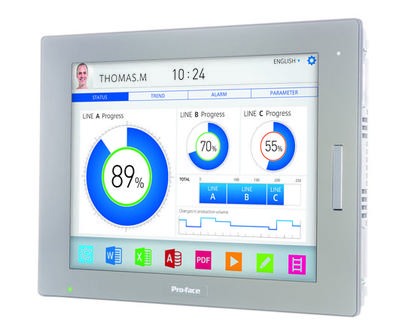
\includegraphics[width=\linewidth, height=.15\textheight,keepaspectratio]{images/ecranIHM}
  \end{subfigure}%
%
  \begin{subfigure}{0.49\textwidth}
    \centering
    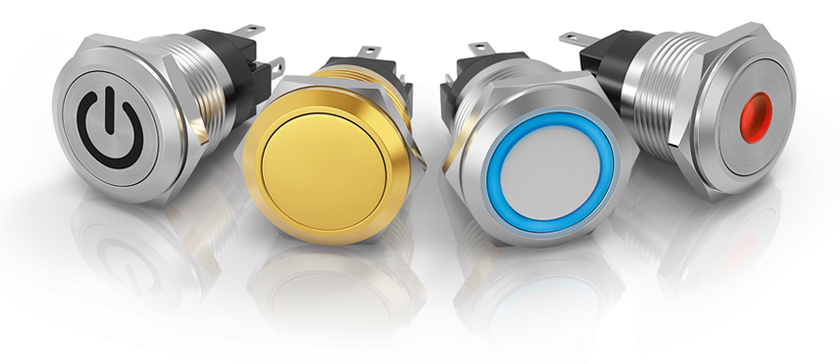
\includegraphics[width=\linewidth,height=.15\textheight,keepaspectratio]{images/boutons}
  \end{subfigure}
  \caption{Ecran et boutons poussoirs pour une IHM}
  \label{fig:IHM}
\end{figure}


